%%%%%%%%%%%%%%%%%%%%%%%%%%%%%%%%%%%%%%%%%
% Short Sectioned Assignment
% LaTeX Template
% Version 1.0 (5/5/12)
%
% This template has been downloaded from:
% http://www.LaTeXTemplates.com
%
% Original author:
% Frits Wenneker (http://www.howtotex.com)
%
% License:
% CC BY-NC-SA 3.0 (http://creativecommons.org/licenses/by-nc-sa/3.0/)
%
%%%%%%%%%%%%%%%%%%%%%%%%%%%%%%%%%%%%%%%%%

%----------------------------------------------------------------------------------------
%	PACKAGES AND OTHER DOCUMENT CONFIGURATIONS
%----------------------------------------------------------------------------------------

\documentclass[paper=a4, fontsize=12pt]{scrartcl} % A4 paper and 11pt font size

\usepackage[margin=1.0in]{geometry}

\usepackage[T1]{fontenc} % Use 8-bit encoding that has 256 glyphs
\usepackage{fourier} % Use the Adobe Utopia font for the document - comment this line to return to the LaTeX default
\usepackage[english]{babel} % English language/hyphenation
\usepackage{amsmath,amsfonts,amsthm} % Math packages

\usepackage{lipsum} % Used for inserting dummy 'Lorem ipsum' text into the template

\usepackage{sectsty} % Allows customizing section commands
\allsectionsfont{\centering \normalfont\scshape} % Make all sections centered, the default font and small caps

\usepackage{IEEEtrantools}
\usepackage{listings}
\usepackage{caption}
\usepackage{subcaption}
\usepackage{graphicx}
\usepackage{mathtools}

\usepackage{fancyhdr} % Custom headers and footers
\pagestyle{fancyplain} % Makes all pages in the document conform to the custom headers and footers
\fancyhead{} % No page header - if you want one, create it in the same way as the footers below
\fancyfoot[L]{} % Empty left footer
\fancyfoot[C]{} % Empty center footer
\fancyfoot[R]{\thepage} % Page numbering for right footer
\renewcommand{\headrulewidth}{0pt} % Remove header underlines
\renewcommand{\footrulewidth}{0pt} % Remove footer underlines
\setlength{\headheight}{13.6pt} % Customize the height of the header

\numberwithin{equation}{section} % Number equations within sections (i.e. 1.1, 1.2, 2.1, 2.2 instead of 1, 2, 3, 4)
\numberwithin{figure}{section} % Number figures within sections (i.e. 1.1, 1.2, 2.1, 2.2 instead of 1, 2, 3, 4)
\numberwithin{table}{section} % Number tables within sections (i.e. 1.1, 1.2, 2.1, 2.2 instead of 1, 2, 3, 4)

%\setlength\parindent{0pt} % Removes all indentation from paragraphs - comment this line for an assignment with lots of text

%----------------------------------------------------------------------------------------
%	TITLE SECTION
%----------------------------------------------------------------------------------------

\newcommand{\horrule}[1]{\rule{\linewidth}{#1}} % Create horizontal rule command with 1 argument of height

\title{	
\normalfont \normalsize 
\textsc{Department of EE - IIT Madras} \\ [25pt] % Your university, school and/or department name(s)
\horrule{0.5pt} \\[0.4cm] % Thin top horizontal rule
\huge Assignment 6 \\Spatial Coupling and Threshold Saturation % The assignment title
\horrule{2pt} \\[0.5cm] % Thick bottom horizontal rule
}

\author{Surajkumar Harikumar (EE11B075)} % Your name

\date{\normalsize\today} % Today's date or a custom date

\begin{document}

\maketitle % Print the title

%----------------------------------------------------------------------------------------
%	PROBLEM 1
%----------------------------------------------------------------------------------------

\section{Problem Statement}

Compute the uncoupled threshold for a protograpgh code. Compute the Area threshold of the spatially coupled extension of the code, and compare the two. 

\section{Spatial Coupling}

Here, we use the Protograph code $[3,3]$, that is 2 variable nodes of degree 3 connected to a single check node of degree 6. This is a rate-$\frac{1}{2}$ code. A horizontally repeated version of the protograph code is shown in Figure (\ref{fig:uncoup}). The spatially coupled version of this code involves spreading the edges of the protograph among its nearest neighbours. At the terminal nodes, we add extra check nodes to complete the chain. Figure (\ref{fig:coup}) shows the coupled version of the same $[3,3]$ code.  

\begin{figure*}
        \centering
        \begin{subfigure}{.5\textwidth}
  \centering
        
\includegraphics[width=0.8\linewidth]{images/tc2}
                \caption{Uncoupled Code}
                \label{fig:uncoup}
                \end{subfigure}%
\begin{subfigure}{.5\textwidth}
  \centering
        
\includegraphics[width=0.8\linewidth]{images/tc1}
                \caption{Coupled Code}
                \label{fig:coup}
	\end{subfigure}
            
\caption{Uncoupled and Coupled versions of the Base  Protograph Code}
\label{fig:qq}            
\end{figure*}

Spatially coupled protographs have a higher threshold than their base protograph (under BP decoding). We first motivate this claim, and then give the method to find the new threshold. Say we are operating just above the BP threshold. We look only at the terminal nodes, and ignore the information from the rest of the graph. 

This forms a small protograph by itself, and can be decoded (if below its threshold). Since every node is connected only to its neighbours, we can propagate this decoded information like a wave throughout the rest of the graph, allowing stage-wise decoding. 

To compute the threshold, we can plot the EXIT-chart under BP decoding. The BP-threshold $\epsilon_{BP}$ is computed using methods from the earlier assignment. The threshold is the $\epsilon$ which causes the 2-EXIT curves to touch. For the spatially coupled code, we allow the 2 curves to intersect. We compute the \textbf{Area Threshold} $\epsilon_{Area}$ as the $\epsilon$ which causes the areas to be equal. \\ \\
An alternative formulation is to define a potential function for spatially coupled codes as
\begin{equation}
U(x,\epsilon) = \int_0^x \left(z-\epsilon \lambda \left(1-\rho\left( 1-z\right)\right)\right)\rho' (1-z) dz
\end{equation}

It has been shown in \cite{EPFL}, that $\epsilon_{Area}$ causes the potential function to touch $U(x)=0$ at exactly one non-zero point, and stays positive. This provides an easy way to compute the area threshold for any protograph. The authors also show $\epsilon_{Area}$ corresponds to the MAP threshold for the protograph. 

\section{Threshold Calculation}

To find the BP threshold, we use \textbf{proto\_thresh\_bec\_brute.m} from Assignment 3. The code we use has $\lambda(x)=x^2; \rho(x)=x^5$. For this protograph, $\epsilon_{BP}=0.4294$. The Potential function based threshold computation is implemented in the script \textbf{spatcoup.m}.

Figure (\ref{spat}) shows a plot of the potential function for various values of $\epsilon$. For this spatially coupled protograph, $\epsilon_{Area}=0.48815$

\begin{figure}[h]
\centering
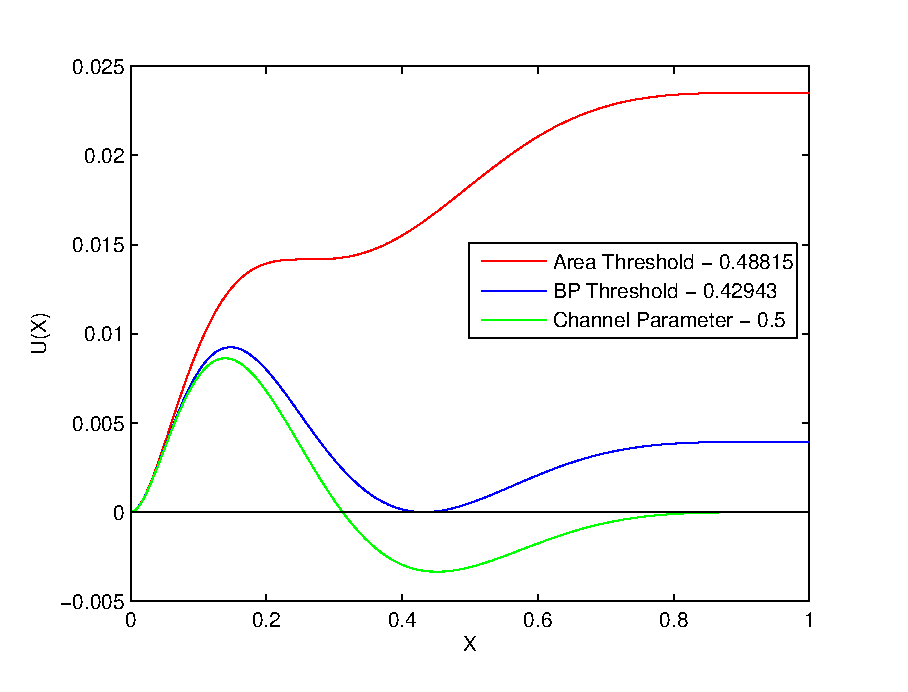
\includegraphics[width=0.8\textwidth]{images/spat}
\caption{Potential Function plot for various values of $\epsilon$}
\label{spat}
\end{figure}

\section{Capacity Achieving}

\begin{figure}
\centering
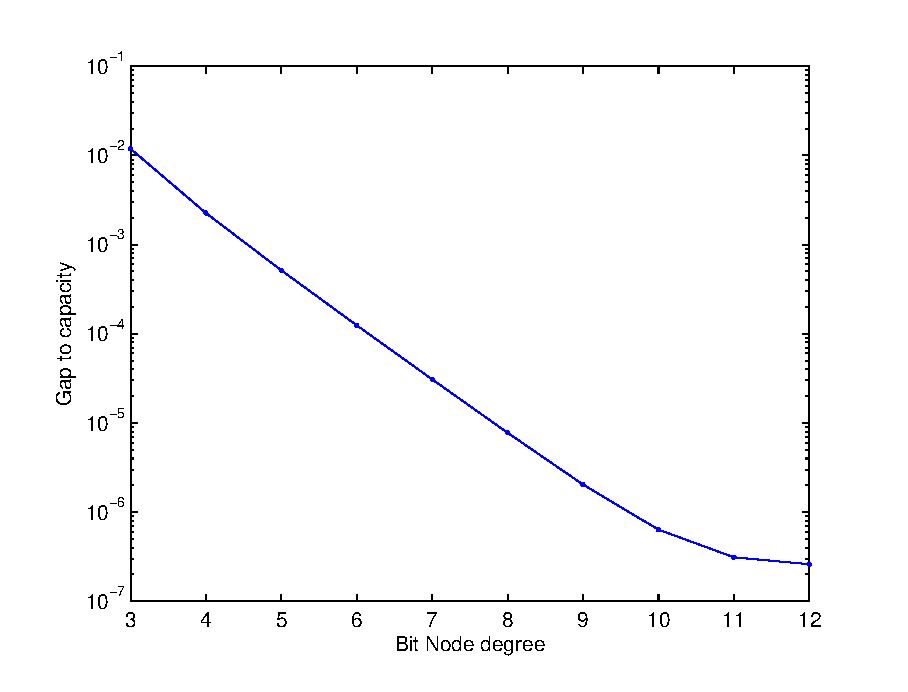
\includegraphics[width=0.8\textwidth]{images/capacity}
\caption{Gap to capacity as a function of bit-node degree}
\label{capacity}
\end{figure}

Kudekar et.al \cite{Capacity} have shown that Spatially Coupled codes can achieve capacity. We construct a sequence of spatially coupled codes of increasing bit-node degree. The check node degree is $2x$ the bit-node degree. We compute the Area threshold for every such protograph. The script to implement this is \textbf{spatcoup\_capacity.m}

Figure (\ref{capacity}) shows how the Gap to Capacity varies with the bit-node degree of the spatially coupled code. The Gap to capacity here is $0.5-\epsilon_{Area}$. We observe an exponential fall in the Gap to capacity with increasing bit-node degree. The saturation-like behaviour at the bottom is from MATLAB precision effects, and can be remedied by taking more sample points. As the node degrees tend to infinity in a spatially coupled code, the threshold appears to approaches capacity. 


\begin{thebibliography}{300}
\bibitem{EPFL}
EPFL tutorial on Spatially Coupled codes, \textit{ISIT 2013} - \\
http://ipg.epfl.ch/doku.php?id=en:publications:scc\_tutorial

\bibitem{Capacity}
S. Kudekar, T. Richardson, R. Urbanke; \textit{Spatially Coupled Ensembles Universally Achieve Capacity under Belief Propagation} - http://arxiv.org/abs/1201.2999

\bibitem{Imger}
Images used in Figure \ref{fig:qq} - \\
http://ita.ucsd.edu/wiki/index.php?title=Spatially\_coupled\_codes

\end{thebibliography}
\end{document}

